%; whizzy paragraph -pdf xpdf -latex ./whizzypdfptex.sh
%; whizzy-paragraph "^\\\\begin{frame}\\|\\\\emtext"
% latex beamer presentation.
% platex, latex-beamer $B$G%3%s%Q%$%k$9$k$3$H$rA[Dj!#(B 

%     Tokyo Debian Meeting resources
%     Copyright (C) 2012 Junichi Uekawa

%     This program is free software; you can redistribute it and/or modify
%     it under the terms of the GNU General Public License as published by
%     the Free Software Foundation; either version 2 of the License, or
%     (at your option) any later version.

%     This program is distributed in the hope that it will be useful,
%     but WITHOUT ANY WARRANTY; without even the implied warreanty of
%     MERCHANTABILITY or FITNESS FOR A PARTICULAR PURPOSE.  See the
%     GNU General Public License for more details.
%     You should have received a copy of the GNU General Public License
%     along with this program; if not, write to the Free Software
%     Foundation, Inc., 51 Franklin St, Fifth Floor, Boston, MA  02110-1301 USA

\documentclass[cjk,dvipdfmx,12pt]{beamer}
\usetheme{Tokyo}
\usepackage{monthlypresentation}

%  preview (shell-command (concat "evince " (replace-regexp-in-string "tex$" "pdf"(buffer-file-name)) "&")) 
%  presentation (shell-command (concat "xpdf -fullscreen " (replace-regexp-in-string "tex$" "pdf"(buffer-file-name)) "&"))
%  presentation (shell-command (concat "evince " (replace-regexp-in-string "tex$" "pdf"(buffer-file-name)) "&"))

%http://www.naney.org/diki/dk/hyperref.html
%$BF|K\8l(BEUC$B7O4D6-$N;~(B
\AtBeginDvi{\special{pdf:tounicode EUC-UCS2}}
%$B%7%U%H(BJIS$B7O4D6-$N;~(B
%\AtBeginDvi{\special{pdf:tounicode 90ms-RKSJ-UCS2}}

\newenvironment{commandlinesmall}%
{\VerbatimEnvironment
  \begin{Sbox}\begin{minipage}{1.0\hsize}\begin{fontsize}{8}{8} \begin{BVerbatim}}%
{\end{BVerbatim}\end{fontsize}\end{minipage}\end{Sbox}
  \setlength{\fboxsep}{8pt}
% start on a new paragraph

\vspace{6pt}% skip before
\fcolorbox{dancerdarkblue}{dancerlightblue}{\TheSbox}

\vspace{6pt}% skip after
}
%end of commandlinesmall

\title{go / debian $B$G$N5!3#3X=,4D6-9=C[$K$D$$$F(B}
\author{$Bc7F#(B $BM:2p(B  ysaito@golangcoder.club}
\date{2018$BG/(B3$B7n(B24$BF|(B}
\logo{
\includegraphics[width=8cm]{image200607/openlogo-light.eps}}

\begin{document}

\begin{frame}
\titlepage{}
\end{frame}

\begin{frame}{$B;29M$K$7$?;qNA(B}
  Machine Learning with Go (packt publishing)
  %%BoundingBox: 0.00 0.00 362.83 272.13
  
\includegraphics[width=0.8\hsize]{image201803/Shiryo001.png}
\end{frame}


\section{}
%\emtext{}

\begin{frame}[containsverbatim]{$BEA$($?$$$3$H(B}
$B5!3#3X=,$H$$$&$H(B python $B$d(B R $B$,A*Br;h$K$"$,$k$,(B,
Go $B$K$h$k5!3#3X=,4D6-9=C[$b%a%j%C%H$,$"$j$=$&(B
\begin{itemize}
 \item $B@EE*7?0BA4(B
 \item $BJBNs7W;;(B
 \item $B%]!<%?%S%j%F%#$d(B, $B%7%9%F%`%W%m%0%i%_%s%0$H$N?FOB@-(B
\end{itemize}

\end{frame}

\begin{frame}{$B9=C[$9$k4D6-35MW(B}

%%BoundingBox: 0.00 0.00 362.83 272.13
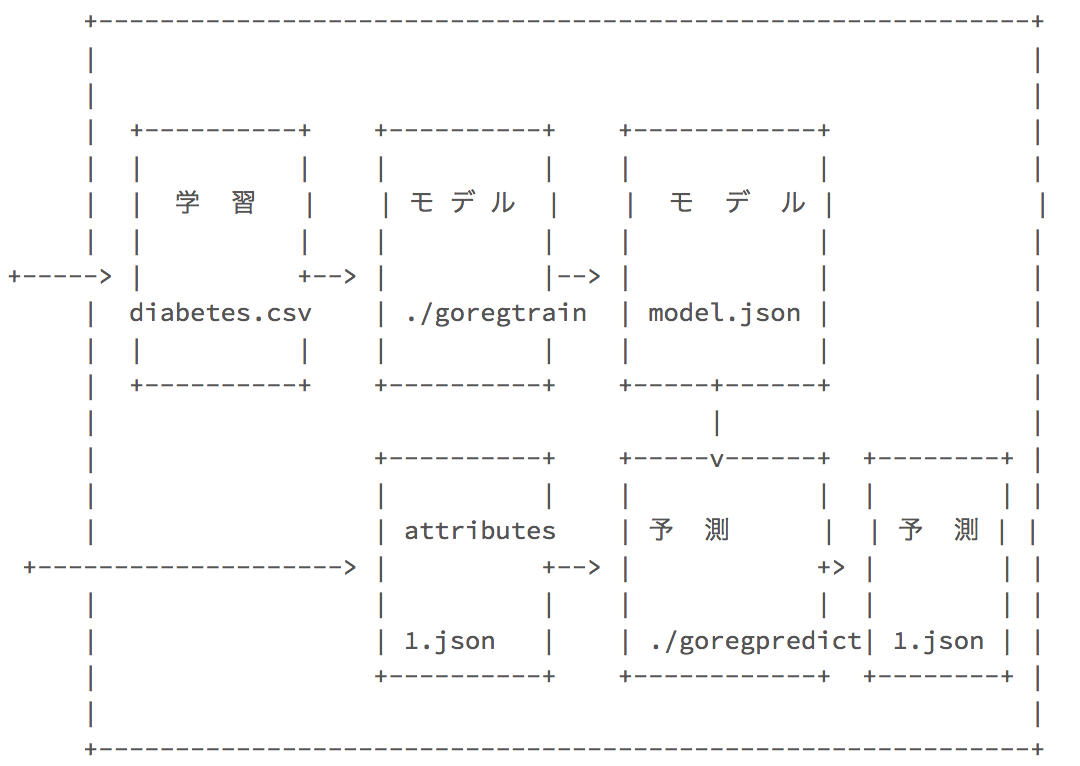
\includegraphics[width=0.8\hsize]{image201803/Shiryo002.png}

\end{frame}

\begin{frame}{debian $B$G9=C[$9$kF05!(B}

rasbian $B$G9=C[$G$-$l$P(B,
raspberry pi $B$r$D$J$2$F(B, $B%/%i%9%?$,:n$j$d$9$$$N$G$O(B!

\end{frame}

\begin{frame}{$BF3F~$9$k%D!<%k(B}

\begin{itemize}
 \item kubernetes : $B%3%s%F%J%*!<%1%9%H%l!<%7%g%s%D!<%k(B ($B:#2s$O(B minikube)
 \item docker    : $B%3%s%F%J%D!<%k(B
 \item pachyderm : $B%G!<%?%P!<%8%g%K%s%0(B, $B%G!<%?%Q%$%W%i%$%s%D!<%k(B
\end{itemize}

\end{frame}

\end{document}

;;; Local Variables: ***
;;; outline-regexp: "\\([ 	]*\\\\\\(documentstyle\\|documentclass\\|emtext\\|section\\|begin{frame}\\)\\*?[ 	]*[[{]\\|[]+\\)" ***
;;; End: ***
